% Figure 1: Four-Stage Evolution Overview
\documentclass[tikz,border=10pt]{standalone}
\usepackage{tikz}
\usetikzlibrary{shapes,arrows,positioning,calc,fit,backgrounds,shadows}

\begin{document}
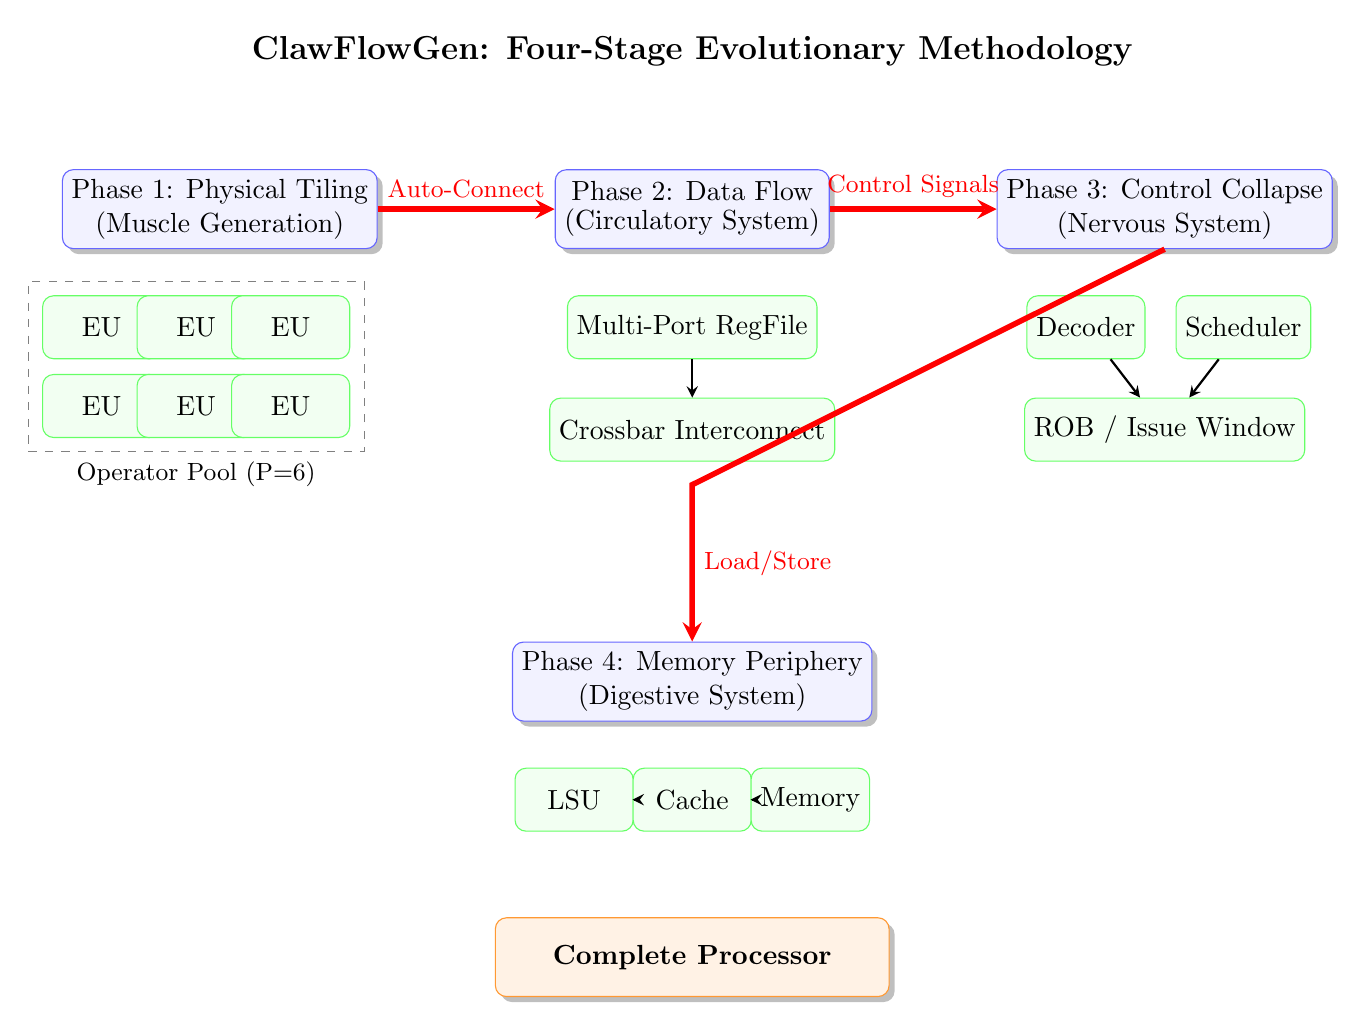
\begin{tikzpicture}[
    node distance=1.5cm,
    box/.style={rectangle, rounded corners, draw=blue!60, fill=blue!5, 
                minimum width=3cm, minimum height=1cm, text centered,
                drop shadow={shadow xshift=2pt, shadow yshift=-2pt}},
    smallbox/.style={rectangle, rounded corners, draw=green!60, fill=green!5,
                     minimum width=1.5cm, minimum height=0.8cm, text centered},
    arrow/.style={->, >=stealth, thick},
    label/.style={font=\bfseries\large}
]

% Title
\node[label] at (0, 6) {ClawFlowGen: Four-Stage Evolutionary Methodology};

% Phase 1: Physical Tiling
\node[box] (phase1) at (-6, 4) {\shortstack{Phase 1: Physical Tiling\\(Muscle Generation)}};
\foreach \i in {0,1,2} {
    \foreach \j in {0,1} {
        \node[smallbox] (eu_\i_\j) at (-7.5+\i*1.2, 2.5-\j*1) {EU};
    }
}
\node[fit=(eu_0_0)(eu_2_1), draw=gray, dashed, inner sep=5pt] (eu_pool) {};
\node[below] at (eu_pool.south) {\small Operator Pool (P=6)};

% Phase 2: Data Flow
\node[box] (phase2) at (0, 4) {\shortstack{Phase 2: Data Flow\\(Circulatory System)}};
\node[smallbox, minimum width=2.5cm] (rf) at (0, 2.5) {Multi-Port RegFile};
\node[smallbox, minimum width=2.5cm] (xbar) at (0, 1.2) {Crossbar Interconnect};
\draw[arrow] (rf) -- (xbar);

% Phase 3: Control
\node[box] (phase3) at (6, 4) {\shortstack{Phase 3: Control Collapse\\(Nervous System)}};
\node[smallbox] (decoder) at (5, 2.5) {Decoder};
\node[smallbox] (scheduler) at (7, 2.5) {Scheduler};
\node[smallbox, minimum width=2.5cm] (rob) at (6, 1.2) {ROB / Issue Window};
\draw[arrow] (decoder) -- (rob);
\draw[arrow] (scheduler) -- (rob);

% Phase 4: Memory
\node[box] (phase4) at (0, -2) {\shortstack{Phase 4: Memory Periphery\\(Digestive System)}};
\node[smallbox] (lsu) at (-1.5, -3.5) {LSU};
\node[smallbox] (cache) at (0, -3.5) {Cache};
\node[smallbox] (mem) at (1.5, -3.5) {Memory};
\draw[arrow] (lsu) -- (cache);
\draw[arrow] (cache) -- (mem);

% Arrows between phases
\draw[arrow, color=red, line width=2pt] (phase1.east) -- (phase2.west) 
    node[midway, above, font=\small] {Auto-Connect};
\draw[arrow, color=red, line width=2pt] (phase2.east) -- (phase3.west)
    node[midway, above, font=\small] {Control Signals};
\draw[arrow, color=red, line width=2pt] (phase3.south) -- (0, 0.5) -- (phase4.north)
    node[midway, right, font=\small] {Load/Store};

% Final processor
\node[box, fill=orange!10, draw=orange!80, minimum width=5cm] (processor) at (0, -5.5) {
    \textbf{Complete Processor}
};

\end{tikzpicture}
\end{document}
